\chapter{Analysis and Design}
This chapter gives an overview of the overall system and explains the design choices made. Throughout the project, we explored various methods to implement a real-time augmented reality system for PWUs operating a wheelchair. Naturally, the structure and goals of the project have developed since the interim report, and we review the differences between the initial goals and final product .

\section{Design Overview}
As stated in the requirements, this project consists of three major components:
\begin{itemize}
	\item Human Detection and Direction (HDD)
	\item Object Mapping and Visualization (OMV)
	\item Reactive Control on ARTA
\end{itemize}

\begin{figure}[ht]
	\centering
	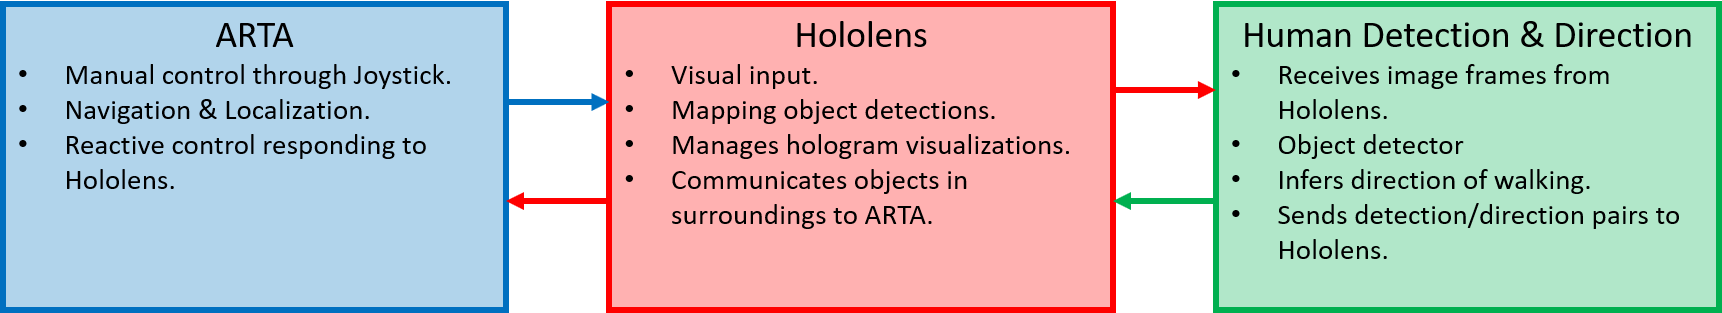
\includegraphics[width=1.0\linewidth]{img/chapter4_analysis/simpleSystemDiagram.png}
	\caption{Simplified high level system diagram}
	\label{fig:simplifiedHL}
\end{figure}

From a very high level view, we can map these requirements to the respective devices they will be operating on. The HDD system takes implements the object detection and human direction inference, while the Hololens is responsible for utilizing the spatial mapping to obtain world positions of the detections, as well as visualizing the detections. The powered wheelchair (ARTA), has manual input that is overridden by the reactive control system that is dependent upon the detections and mappings. The diagram in Figure. \ref{fig:simplifiedHL} shows an overview of the system, and shows that the Hololens acts as an intermediary between ARTA and the HDD.

\subsection{Hardware}

\begin{table}[ht]
	\centering
	\begin{tabular}{l|l|l|l|}
		\cline{2-4}
		& \multicolumn{1}{c|}{\textbf{ARTA}}                                                 & \multicolumn{1}{c|}{\textbf{Hololens}} & \multicolumn{1}{c|}{\textbf{HDD}}                              \\ \hline
		\multicolumn{1}{|l|}{\textbf{Hardware}}         & \begin{tabular}[c]{@{}l@{}}Powered Wheelchair \\ controlled by Laptop\end{tabular} & Hololens                               & \begin{tabular}[c]{@{}l@{}}Desktop PC \\ with GPU\end{tabular} \\ \hline
		\multicolumn{1}{|l|}{\textbf{Operating System}} & Ubuntu 16.04                                                                       & UWP                                    & Ubuntu 16.04                                                   \\ \hline
	\end{tabular}
	\caption{Hardware description of system}
	\label{tab:hardware}
\end{table}

Table. \ref{tab:hardware} summarises the hardware overall system is implemented on. The powered wheelchair, ARTA, is controlled by a laptop, which is responsible for the wheelchair speed, wheel rotations, navigation and localisation. The Hololens is a self contained augmented reality headset, running the Universal Windows Platform (UWP) operating system. Finally, the Human Detection \& Direction system is implemented on a desktop computer with a GTX 1050Ti GPU, allowing it to run real time object detectors.

\subsection{System 
	Communication}

\subsubsection{Robotic Operating System} Since the project spans multiple operating systems, we have chosen to utilize the Robotic Operating System (ROS) as a means of communication between the devices. In ROS, a \textit{node} is defined as a process that performs a computation. A node can be made up of smaller nodes that perform specific computations that serve the needs of the parent node. 

\begin{figure}[ht]
	\centering
	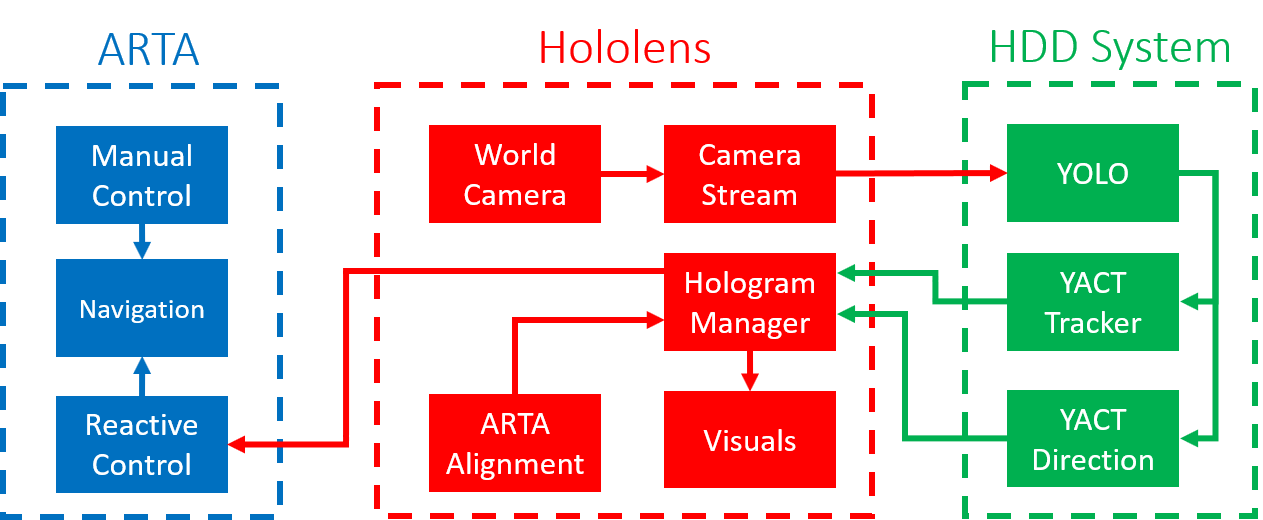
\includegraphics[width=1.0\linewidth]{img/chapter4_analysis/detailedSystemDiagram.png}
	\caption{System diagram detailing individual components}
	\label{fig:detailedHL}
\end{figure}

We can think of the three major systems as large ROS nodes that consists of smaller nodes that run individiual tasks, such as creating the camera stream, or detecting objects. We visualize the breakdown of the system into nodes in Figure. \ref{fig:detailedHL}.

\paragraph{ROS Topics} Nodes in ROS communicate with one another by publishing data in the form of \textit{messages} which get broadcasted over a \textit{topic}. Nodes can choose what data they receive by subscribing to topics. This method allows for nodes running on different devices to communicate with each other, regardless of the operating system. The nodes are unaware that the data it receives is published from a node running on a seperate computer, making ROS a perfect choice for communication in this design.

\section{Human Detection \& Direction System}
The HDD system is reponsible for detecting and predicting the directions of people in the surroundings of the wheelchair. By taking visual inputs in the form of images from the Hololens, we run an object detector trained on a dataset of pedestrians to detect people and heads. The bounding boxes produced by the object detector are fed as inputs to an object tracker and a body pose estimator. We use the results of these two nodes to infer the direction a detected person is moving in, and publish the results back to the Hololens.

\begin{figure}[ht]
	\centering
	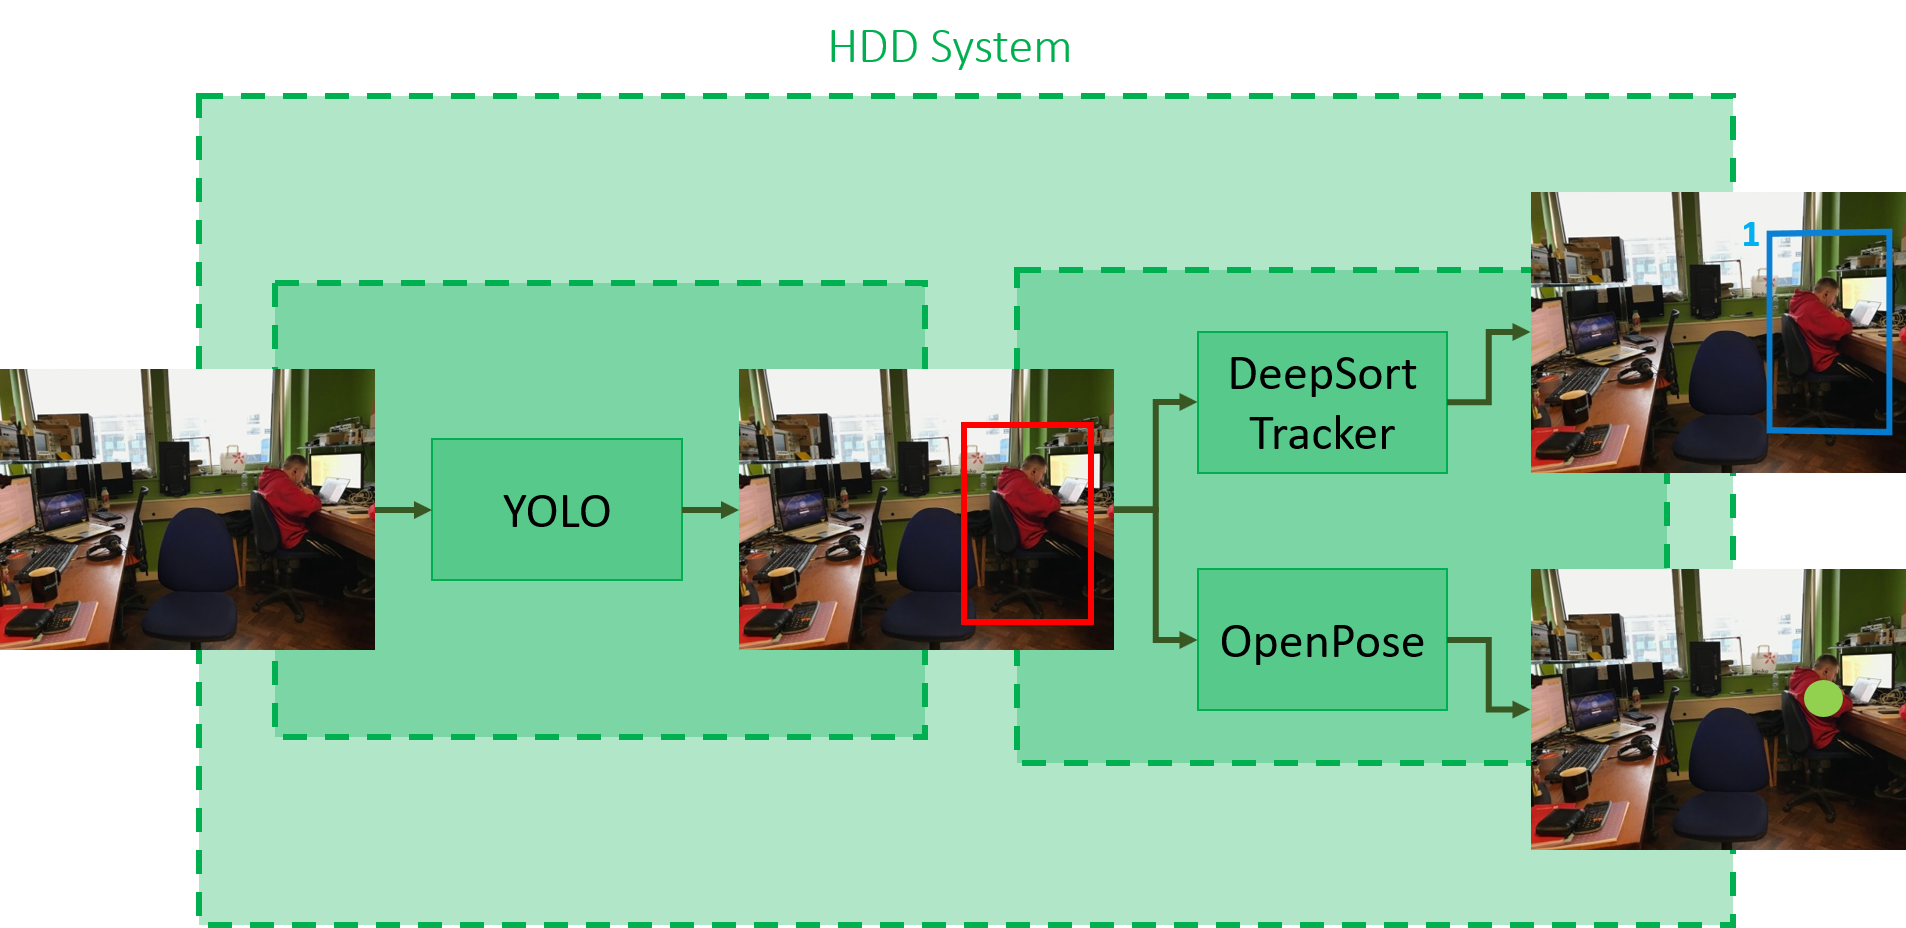
\includegraphics[width=1.0\linewidth]{img/chapter4_analysis/hddSystemDiagram.png}
	\caption{Individual nodes in HDD System}
	\label{fig:detailedHDD}
\end{figure}

We present an overall view of the HDD System, covering the purpose and design of individual components. We also propose the reasoning behind certain design choices, which we cover in more depth later in this report.

\subsection{YOLO Object Detector}
Object detectors often form the input to an object tracker or pose estimation system \cite{Bewley2016, Jin2017}. In the case of top-down body pose estimation methods, detections can be the first point of failure \cite{Insafutdinov}. As such, the accuracy of the chosen object detector must be considered, together with the choice of using a pre-trained model or training on a more relevant dataset. Finally, we must also consider the use-case of the detector, which must be able to operate in real-time and detect moving objects as they pass by.

\subsubsection{Choice of Detector}
As commented on in Section \ref{sec:detector}, modern deep learning techniques outperform classical object detectors in accuracy, but are limited by the requirement of a GPU to perform in real-time. Since the Hololens does not have built in support to run object detection networks, Microsoft provides the Azure Cognitive Services API to allow developers to query their system for object detections. The limitation is that this service is not free, and abstracts away the implementation of an object detector. Furthermore, one of the personal goals for this project was to learn more about CNNs in computer vision.

\paragraph{} Taking this into account, we compared several deep learning architectures for object detection. Previous work done in the PRL used Facebook AI Research's (FAIR) Detectron to detect objects \cite{Chacon-Quesada, Detectron2018, Rena}. Further discussions with members of the Imperial Computer Vision \& Learning Lab suggested the use of the YOLO object detector \cite{Redmon}, due to its speed and having a lightweight implementation that could be run on lower end GPUS at relatively high frame rates. This prompted the design decision to use the Darknet framework to run the \textbf{YOLOv3-tiny} architecture as the object detection method of choice for this project \cite{Redmon2018}.

\subsubsection{Pre-trained Model vs Training}
An advantage of using the YOLO Darknet framework is that it provides models which are already trained to detect multiple object classes, including the class \textit{Person}. One of the pre-trained models is the YOLOv3-tiny architecture trained on the Common Objects in Context (COCO) dataset \cite{Lin}.

\paragraph{Comparing Models} To compare the accuracy of the bounding boxes produced by pre-trained model, sample videos were recorded using the Hololens and used as a base comparison point. It was quickly shown that although the COCO trained model can detect individuals, or multiple people who are well spaced out, it had difficulty in differentiating between people who are close together or slighlty occluded. Figure \ref{fig:yoloCHvsCoco} highlights the issue of the COCO model failing to detect small people close together.

\begin{figure}[ht]
	\begin{subfigure}[b]{.5\textwidth}
		\centering
		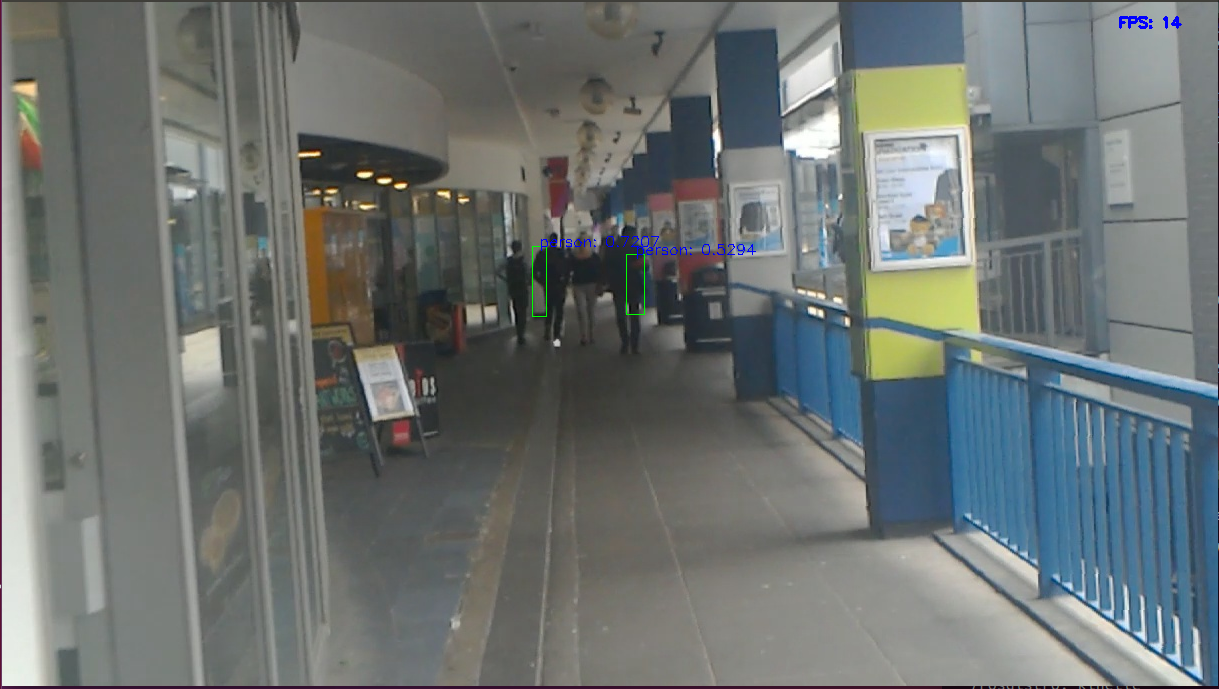
\includegraphics[width=1.0\linewidth]{img/chapter4_analysis/yoloCoco.png}
		\caption{COCO YOLOv3-tiny}
	\end{subfigure}%
	\hspace{\fill} 
	\begin{subfigure}[b]{.5\textwidth}
		\centering
		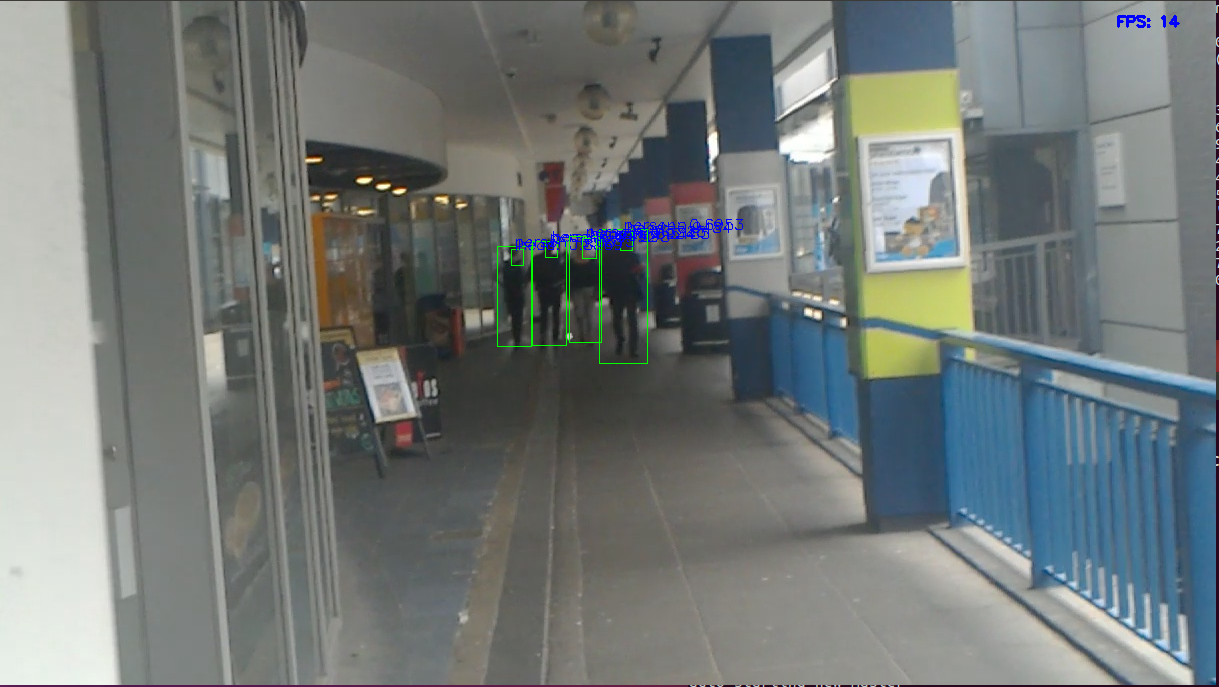
\includegraphics[width=1.0\linewidth]{img/chapter4_analysis/yoloCH.png}
		\caption{Trained YOLOv3-tiny}
	\end{subfigure}
	\vspace{-2\baselineskip}
	\begin{center}
		\caption{Comparison of COCO model and our model trained on a pedestrian dataset.}
		\label{fig:yoloCHvsCoco}
	\end{center}
	\vspace{-2\baselineskip}
\end{figure}

\paragraph{Pedestrian Dataset} A common case in pedestrian detection is occlusion, where only certain body parts are visible.  To resolve this issue, we decided to train the YOLOv3-tiny model on the \textbf{CrowdHuman} dataset \cite{Shao}, which contains annotated images of crowds, including bounding boxes for the head, visible human region and full-body. The annotations for partially visible people allows the network to detect occlusions, solving the issue of people being close to each other. We also trained the network to detect heads, since we initially wanted to use head pose estimation to determine direction.

\subsubsection{Analysis}
The result of training the YOLOv3-tiny model on the CrowdHuman dataset is that the system is able to detect smaller figures who are occluded. We go into further detail on the training process in the Implementation section of this report.

\subsection{YACT: Yet Another Crowd Tracker}

\subsubsection{Object Tracking}

\subsubsection{Body Pose Estimation}

\subsubsection{Head Pose Estimation}

\section{Hololens}
\subsection{Breakdown}

\section{ARTA}
\subsection{Breakdown}


